% !TeX TS-program = pdflatex
\documentclass{beamer}

\usepackage{tikz}
\usetikzlibrary{overlay-beamer-styles}
\setbeamertemplate{navigation symbols}{}

\begin{document}

\begin{frame}<90-930>[plain]%%%%%%%%%%%%%%%%%%%%%%%%%%%%%%%%%%%%%%%%%%%
	\begin{tikzpicture}[remember picture,overlay]
  	\node[at=(current page.center)]{
   		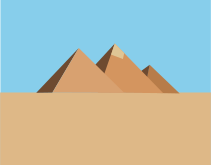
\includegraphics[width=\paperwidth]{pyramids}
		};
  	\node at (10,-4) {
   		\includegraphics[width=2.5cm]{mummy_closedeyes}
		};		
		\foreach \x in {0,0.003,...,3.2}{
			\node<+>[scale=\x] at (12-0.1*22.5*\x*\x,-1.5-0.06*4*\x*\x) {
\includegraphics[height=1.6cm]{stone}};			
		}
	\end{tikzpicture}
\end{frame}

\begin{frame}[plain]%%%%%%%%%%%%%%%%%%%%%%%%%%%%%%%%%%%%%%%%%%%%%%%%%%
	\begin{tikzpicture}[remember picture,overlay]
  	\node[at=(current page.center)]{
   		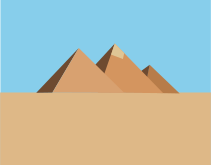
\includegraphics[width=\paperwidth]{pyramids}
		};
  	\node at (10,-4) {
   		\includegraphics[width=2.5cm]{mummy}
		};		
	\end{tikzpicture}
	\pause[70]
\end{frame}

\end{document}